%!TEX root = ../abgabe.tex

\section{Gestaltung von Applikationen für mobilen Kontext}

Geschrieben von: \textbf{Saulius Archipovas}
\newline

Mit der stetigen Verbreitung von Smartphones und mobilen Geräten im alltäglichen Leben, steigt auch die Benutzung von Applikationen in mobilen Kontexten. Dabei stoßen viele der Benutzer, die mittels ihrem mobilen Gerät auf vorhandene Dienste zugreifen wollen, vielmals auf Usability Probleme. Solche Probleme liegen nicht nur in der Inhaltsstruktur oder der visuelle Kommunikation begründet, sondern auch in Funktionenen, die die Dienste anbieten. Dies liegt zumeist daran, dass diese Dienste für die Erledigung von Aufgaben an einem stationären Rechner konzipiert wurden. So werden speziellen Gegebenheiten von mobilen Geräten, die sowohl Einschränkungen als auch Vorteile, für den Benutzer bedeuten, bei der Entwicklung oftmals nicht beachtet.
Bei schon vorhandenen Applikationen muss daher meistens nicht nur das Design, sondern auch die Funktionalität der Applikationen sowie die Benutzungsumgebung an die Benutzerintentionen angepasst werden. 


In diesem Abschnitt werden verschiedene Gestaltungsprinzipien vorgestellt, die bei der Gestaltung und Entwicklung von Applikationen und Webseiten  für einen mobilen Kontext zu beachten sind. Viele der vorgestellten Prinzipien sind nützlich für eine breite Palette von Geräten, die im mobilen Kontext benutzt werden können. Es wird sich in dieser Ausarbeitung aber vorwiegend auf die Gestaltung von Applikationen für Smartphones in bezogen. In Abschnitt \ref{sub:Benutzerschnittstellen} werden die Prinzipien für den Aufbau wesentlicher Bedienelemente und die Interaktionsmöglichkeiten mit ihnen vorgestellt. Hiernach in Abschnitt \ref{sec:Informationsaufbereitung} werden alternative Möglichkeiten der Informationsarchitektur  aufgezeigt, die bei der Erstellung von Applikationen für mobile Kontexte erwogen werden sollten. Da auch die Dienste bestimmte Anforderungen erfüllen sollten, werden diese im Abschnitt \ref{sub:gestaltung_von_diensten} erläutert. Am Ende dieses Kapitels, werden Gestaltungshinweise für die Entwicklung von Applikationen im Wearable Computing Kontext, die spezielle Anforderungen erfüllen müssen, vorgestellt.

In allen Abschnitten werden keine generellen Gestaltungsprinzipien wie z.B. Gesetze der Nähe vorgestellt. Sondern es wird sich im Wesentlichen auf solche konzentriert, die für den mobilen Kontext als wichtig erscheinen.

\subsection{Bedienelementen und Interaktion}
\label{sub:Benutzerschnittstellen}

Es gibt eine Vielzahl von Smartphones, sowie deren Eingabe- und Ausgabearten. Der Benutzer kann mit einem Gerät über Touchscreen, Tastatur, Ziffernblock, Trackpoint usw. interagieren. Jeder dieser Eingabegarten hat einen anderen Charakter. Es werden folgenden Prinzipien auf die Eingabe mittels Touchscreenbeziehen beziehen, da solche Benutzerschnittstellen sind für Smartphones am meisten beliebt und verbreitet.

\subparagraph{Bedienelementen auf der graphische Oberfläche} 
\label{subp:gro_ere_interface_elementen}

Die Einschränkungen kleiner Bildschirme auf einem Smartphone müssen bei der Erstellung von grafischen Benutzeroberflächen besonders beachtet werden. Zu nennen sind hier etwa die physischen Eigenschaften der Fingerkuppe: Laut einer Studie von MIT Touch Lab, ist die menschliche Fingerkuppe im Durchschnitt etwa 10-14mm breit, und die Fingerspitze etwa 8-10mm\cite{Srinivasan:2003uu}.  Pekka Parhi  et.al haben in ihrer Studie \cite{Parhi:2006gh} erforscht, welche optimale Größe von Bedienungselementen für eine einhändige Daumeninteraktion erforderlich ist: Sie setzen die Mindestgröße für getrennte Aufgaben bei $>$ 9,5 \textit{mm} an.  Bei seriellen Erledigungen von Aufgaben sehen sie $>$ 7.7 \textit{mm}als optimal. Größere Bedienelemente weisen keine signifikant präzisere Erledigung der Aufgaben auf.
Auch die Hersteller von mobilen Betriebssystemen schlagen ähnliche Maße für Bedienelemente vor. Apple setzt eine Mindestgröße von 44 x 44 Punkten \cite{Apple}, Microsoft 7 \textit{mm} oder 26 \textit{px}\cite{lukeGUI} für Elemente voraus.

Nicht nur die Größe der Elemente, sondern auch der Zwischenabstand zwischen ihnen ist wichtig für eine benutzerfreundliche Bedienung der Anwendung. Wie in Abbildung~\ref{fig:login} zu sehen ist, muss der Benutzer sich hier anstrengen, um das richtige Element in der Liste auszuwählen. Auch die Möglichkeit den "Cancel" – Buttons unvorhergesehen anzuklicken, kann in diesem Beispiel vorhersehbar sein (siehe Abbildung~\ref{fig:login}). So ist ein Zwischenabstand zwischen Bedienelementen, der sogenannte Whitespace,  empfohlen. Solche Abstände sollten mindestens von 2\textit{mm} bis 8\textit{px} betragen\cite{lukeGUI} um eine unbeabsichtigte Eingabe zu vermeiden.

\begin{figure}
	\centering
	\begin{subfigure}[b]{0.3\textwidth}
		\centering
		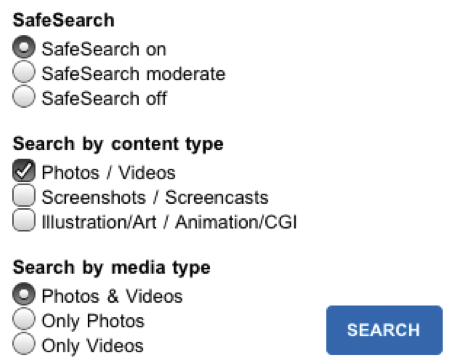
\includegraphics[width=1\textwidth]{img/login.png}
		\caption{Kein Whitespace bei eine Liste, vgl. \cite{mobileFirst}}
		\label{fig:login}
	\end{subfigure}
	\begin{subfigure}[b]{0.6\textwidth}
		\centering
			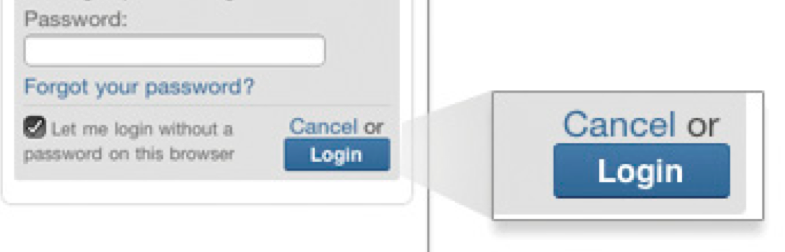
\includegraphics[width=1\textwidth]{img/cancel.png}
	\caption{Kein Whitespace bei Login und Cancel, vgl. \cite{mobileFirst}}\label{fig:cancel}
	\end{subfigure}
	\caption{Positionierung von Elementen}\label{fig:elementPos}
\end{figure}
\subparagraph{Anordnung von Elementen} 
\label{subp:anordnung_von_elementen}

Die richtige Auslegung von Elementen in der Benutzeroberfläche, kann dem Benutzer helfen, ohne hohen Kraftaufwand oder Änderung der Haltung des Geräts auf die wichtigen Funktionen zuzugreifen. Eine einhändige Interaktion mit Smartphones sollte ermöglicht werden, um das Bedienen im mobilen Kontext zu erleichtern. So wird empfohlen, die wichtigen Elemente so auszulegen, dass sie leicht mit dem Daumen erreicht werden können \cite[Seite 209]{mobileFrontier}. Da etwa 70 bis 90 $\%$ der Menschen Rechtshändig sind, ist es laut \cite[Seite 72]{mobileFirst} verbreitet die Elemente nach der Bequemlichkeit für die Daumenbewegung für Rechtshänder in 3 Bereichen auszulegen, wie im Abbildung~\ref{fig:rechtsPositioning} zu sehen ist. Da aber keine Benutzer benachteiligt werden sollen, wurden in dieser Arbeit zusätzlich anhand der Ergebnisse aus der Studie \cite{Park:2010tu} die Bereiche so verändert, dass auch Linkshänder erleichterten Zugriff haben. Das  Resultat wird im Abbildung~\ref{fig:forallPositioning}\cite[Seite 72]{mobileFirst} präsentiert.

Die Bedienungselementen, die sehr oft in der Interaktion benutzt werden, sollten in Bereich "Leicht" platziert werden, da sie leicht mit dem Daumen erreicht werden können. Die Elemente im "Ok" Bereich, brauchen dagegen schon ein wenig mehr Daumenbewegung und bieten weniger Komfort für den Anwender. Der Bereich "Greifen" muss meistens mittels einer Greifbewegung erreicht werden, und bietet sich für Navigationselemente an, nicht so oft verwendet werden.

\begin{figure}
	\centering
	\begin{subfigure}[b]{0.3\textwidth}
		\centering
			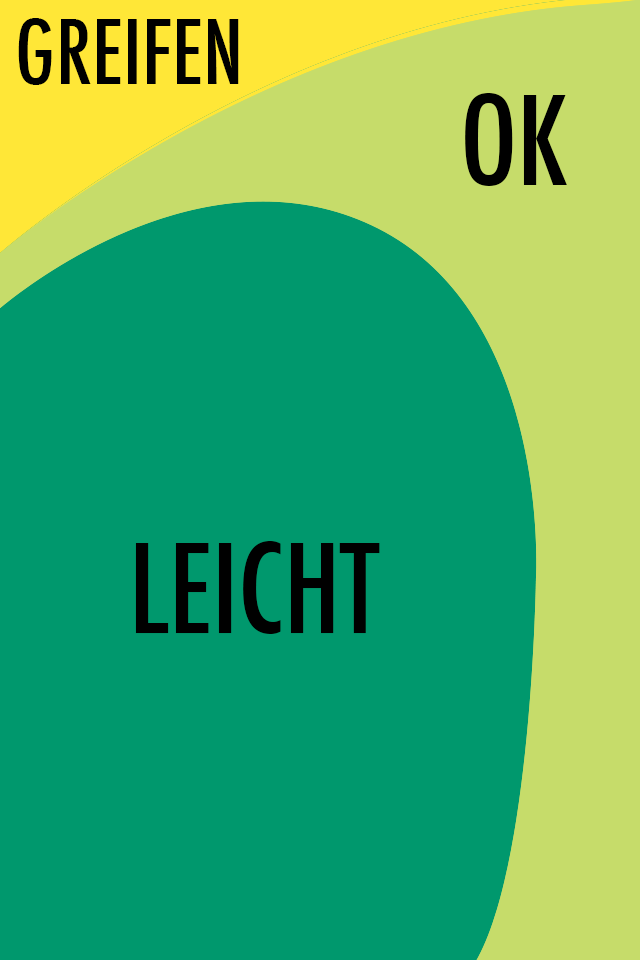
\includegraphics[width=1\textwidth]{img/anordungDerElementeSimple.png}
			\caption{Für Rechtshänder\linebreak}\label{fig:rechtsPositioning}
	\end{subfigure}
	\begin{subfigure}[b]{0.3\textwidth}
		\centering
			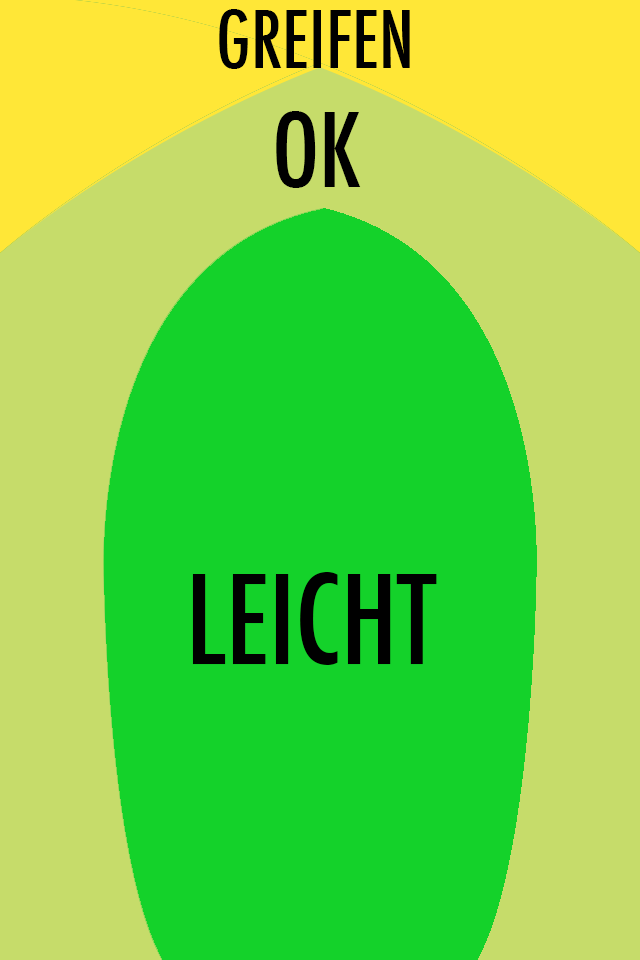
\includegraphics[width=1\textwidth]{img/anordungDerElementeForAll.png}
			\caption{Für Links- und Rechthänder, angepasst anhand Studie \cite{Park:2010tu}}\label{fig:forallPositioning}
			
	\end{subfigure}
	\caption{Positionierung von Elementen}\label{fig:elementPos}
\end{figure}


\subparagraph{Vorsicht bei NUI} 
\label{subp:benutze_nui}

Die meisten Touchgeräte bieten eine direkte Eingabe, mit der natürliche Gesten möglich sind. Dabei läuft man Gefahr, dem Anwender die Bedienbarkeit der Applikation zu erschweren anstatt zu erleichtern. In mobilen Kontexten können viele Situationen auftreten, in denen man nur eine Hand bzw. einen Finger für die Bedienung des Smartphones benutzen kann. Dadurch werden Gesten, für deren Ausführung mehr als ein Finger nötig ist, nicht brauchbar. So sollte man über alternative Möglichkeiten zur Ausführung solcher Interaktionen nachdenken. In Beispiel ~\ref{fig:nuibsp} bietet die vorgeschlagene Benutzeroberfläche\footnote{Ausschnitt aus OpenSteetMap.com} als Alternative für die Pinch oder Spread Gesten einen Schaltknopf. Beim Drücken dieses Schaltknopfes, kann die Karte verkleinert oder vergrößert werden. 

\begin{figure}[h]
	\centering
	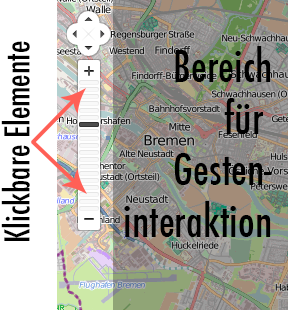
\includegraphics[width=0.3\textwidth]{img/NUIbsp.png}
	\caption{Alternative Bedienelemente für Interaktion}\label{fig:nuibsp}
\end{figure}

\subparagraph{Designe für wechselde Umgebungen} % (fold)
\label{subp:designe_f_r_au_eneinsatz}

In der Bewegung, ändern sich stetig die Umgebungen. Diese haben verschiedene Eigenschaften. So wird zum Beispiel ein Benutzer der aus sonnigem Tageslicht in einen dunklen Kinosaal geht und dabei versucht weiter sein Smartphone zu benutzen, von der starke Leuchtkraft des Bildschirms überblendet. Daher ist es zu empfehlen, solche Bedienelemente leicht erreichbar zu platzieren, die die Helligkeit (vgl. \cite[ff Seite 418]{mobileInteraces}) regulieren. Dementsprechend sollten auch andere Auswirkungen von Umgebungswechseln berücksichtigt werden.

\subsection{Informationsarchitektur}
\label{sec:Informationsaufbereitung}

In diesem Kapitel werden verschiedene Prinzipien für die Informationsarchitektur präsentiert.
Menschen in mobilen Kontexten haben viele Anforderungen an mobile Applikationen. Diese sind anders als für stationäre Arbeitsplätze. Um eine gut benutzbare Software für solchen Szenerien zu entwickeln, ist daher wichtig die Aktionen sowie die Vorlieben des Benutzers zu kennen und dementsprechend auch zu berücksichtigen. Man sollte wissen, warum und wann ein Anwender sein Smartphone im mobilen Kontext benutzt und die Anwendungen auch danach ausrichten.

Jakob Nielsen formuliert in seinem Artikel \footnote{http://www.nngroup.com/articles/mobile-site-vs-full-site/, dies ist ein  Ausschnitt aus dem Bericht "Mobile Website and Application" http://www.nngroup.com/reports/mobile-website-and-application-usability/} generelle Prinzipien, für eine Optimierung der vorhandenen Webseiten für den Gebrauch auf mobilen Geräten:
\begin{itemize}
	\item \textbf{Reduktion der Funktionalität}. So sollen nur Funktionen angeboten werden, deren Anwendungsfall in einen mobilen Kontext passt
	\item \textbf{Beschneidung von Inhalten}, um die Fülle von Text zu verkleinern und um die sekundären Informationen auf anderen Seiten auszulagern
	\item \textbf{Vergrößerung von Elementen auf der Benutzeroberfläche}
\end{itemize}

Allerdings gibt es auch kritische Stimmen, die bezweifeln, dass die Prinzipien von Jakob Nielsen einen richtigen Weg für die Entwicklung von Applikationen für mobile Geräte aufzeigen\footnote{http://www.netmagazine.com/opinions/nielsen-wrong-mobile}. So wird ihm zum Beispiel vorgeworfen, dass man statt der Reduktion von Funktionalitäten die Zusatzmöglichkeiten der mobilen Geräte berücksichtigen solle. Eine Einteilung der Benutzer in verschiedene Kategorien kann dabei helfen, spezielle Wünsche, sowie Erwartungen an die Applikationen herauszufinden.

Die Einteilung, kann laut Google anhand des Anwenderverhaltens vorgenommen werden. Es wurden drei Gruppen identifiziert: "urgent now", "repetitive now", "bored now"\cite{googleUsers}. Benutzer der Gruppe "Urgent now" wollen wenige Informationen schnell bekommen. Ein Beispiel wäre etwa die Adresse eines  Arztes oder Buchladens. Anwendungen, die diese Erwartung erfüllen wollen, sollten etwa mit Hilfe von Ortsdaten, wo sich der Benutzer befindet, die suche initiieren. So sollen die Ergebnisse schnell und ohne bewusste Benutzereingabe geliefert werten. Benutzer der Gruppe "Repretitve now" wollen die gleiche Art von Informationen, wie etwa die Wettervorhersage oder Aktienkurse, immer wieder aufrufen. Solche Informationen sollten schnell sichtbar oder aufrufbar sein. Benutzer die der Gruppe "bored now" angehören, sind oft in einem Zustand, wo sie viel Zeit für die Interaktion mit dem Gerät haben, etwa in der Empfangshalle vom Flughafen oder in öffentlichen Verkehrsmitteln. Die Erwartungen der Benutzer in diese Situationen ähnelt denen der Benutzer, die mit einem stationären Rechner ihre Aufgaben erledigen. Allerdings verfügt der Benutzer im mobilen Kontext über andere Ausgabe- sowie Eingabegeräte und kann so jederzeit für unbestimmte Zeit von der Bedienung des Gerätes unterbrochen werden. So können in einem "bored now" Szenario Aufgaben erledigt werden, die mehr Zeit und kognitive Auslastung voraussetzen, als bei "urgent now" oder "repetitive now".

Die Vorgestellte Einteilung ist zwar nützlich, aber nicht gründlich genug. Daher kann man auch eine Einteilung anhand von Arten der Interaktion statt des Benutzerverhalten vornehmen. Sie ist hilfreicher, um einem Fokus auf die Gestaltung der Informationsarchitektur zu bekommen. Die  Arten von Interaktionen im mobilen Kontext können in vier Kategorien eingeteilt werden( anhand \cite[Seite 50]{mobileFirst}):

\begin{description}
 	\item[Suche (wichtige Information, lokal)] Ich brauche schnell eine Antwort zu meiner Frage. Sie kann auch oft wiederholt vorkommen, und ist bezogen auf meine Position in der Welt
 	\item[Erforschen/Spielen (gelangweilt, lokal)] Ich habe Zeit, und will eine kurze Ablenkung
 	\item[Einchecken/Status (Wiederholung/kleine Aufgaben)] Irgendwas ändert sich, und will ich das Neuste wissen oder teilen
 	\item[Editieren/Kreieren (plötzliche Veränderungen/kleine Aufgaben)] Ich muss schnell etwas erledigen
 \end{description} 

Diese Kategorisierung anhand von Arten der Benutzerinteraktion hilft dessen Bedürfnissen zu erspüren und somit eine auf den Benutzer abgestimmte Applikation zu gestalten. Will man etwa eine Applikation für Wetteraussichten gestalten, so kann man die Benutzer mit Intentionen der Kategorie \textbf{Suche} bedienen, indem man auf dem Startbildschirm das Wetter anhand der lokalen Position des Benutzers anzeigt. Um die Gruppe "Einchecken/Status" zu bedienen, sollte man auch die Möglichkeit bieten, dem Benutzer das Wetter für von ihm abgespeicherte Städten anzuzeigen. Die Gruppe "Erforschen/Spielen", sollte Zusatzfunktionen wie einen 14 Tage Wetterbericht, eine Regenkarte anbieten, die durch Navigation von dem Startbildschirm erreicht werden können.

Es gibt auch generelle Ideen, die eine vorhandene Applikation für den mobilen Kontext optimieren oder neue Applikation gestalten oder umorganisieren können. In folgenden Unterkapiteln werden die wichtigsten Ideen präsentiert. 

\subparagraph{Mach es schlank} 
\label{subp:entferne_das_fett}

Wie schon weiter vorne erwähnt wurde, empfiehlt Jakob Nielsen, die Informationsangebote auf mobilen Webseiten zu reduzieren. So soll unnötiger Text entweder auf anderen Seiten verlagert, oder am besten weggestrichen werden, da sie auf kleinen Geräten schwierig zu lesen sind. \cite[Seite 102]{Nielsen:2012wj}. So muss der Benutzer ständig blättern, braucht mehr Zeit zum Lesen und es ist auch schwieriger zu Textpassagen vor- oder zurück zu springen.

Auch die Funktionsangebote sollen für den mobilen Kontext angepasst werden. Als Beispiel kann hier die Amazon Webseite dienen (siehe Abbildung~\ref{fig:amazon}. So wird bei der Auswahl von einem Produkt auf der mobilen Webseite von Amazon, ein Bild, der Preis und die Möglichkeit für einen sofortigen Kaufen oder den Artikel zu Merken angeboten. Im Vergleich zu einer Desktop Webseite ist das  Funktionsangebot reduziert (siehe Abbildung~\ref{fig:amazonFull}). Um mehr Informationen über das Produkt zu bekommen, was für die Gruppe "Erforschen/Spielen" wurden diese auf sekundäre Seiten ausgelagert

\begin{figure}
	\centering
	\begin{subfigure}[b]{0.3\textwidth}
		\centering
		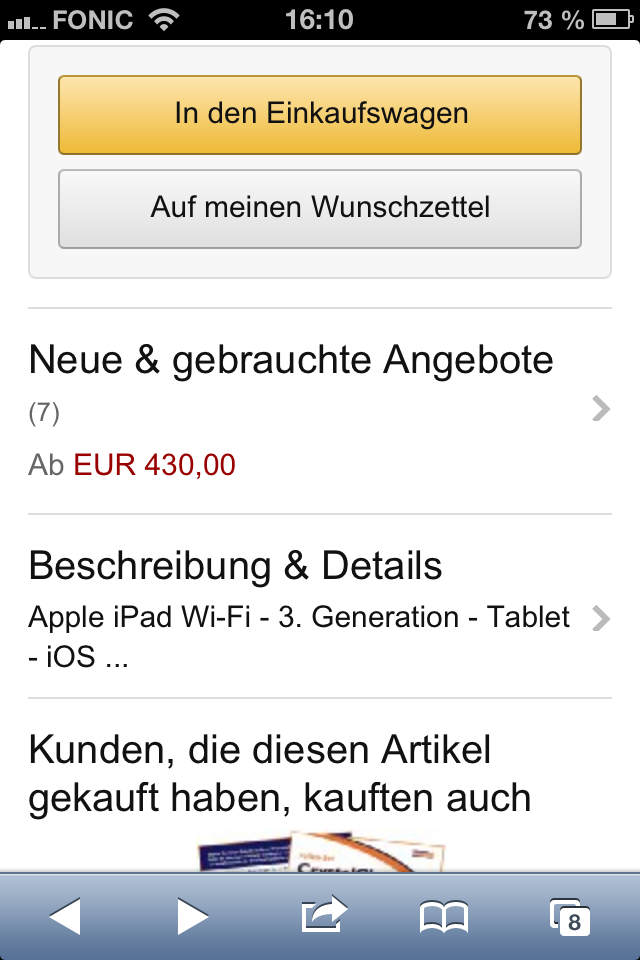
\includegraphics[width=1\textwidth]{img/amazon.png}
		\caption{Mobile Webseite von Amazon}\label{fig:amazon}
	\end{subfigure}
	\begin{subfigure}[b]{0.6\textwidth}
		\centering
		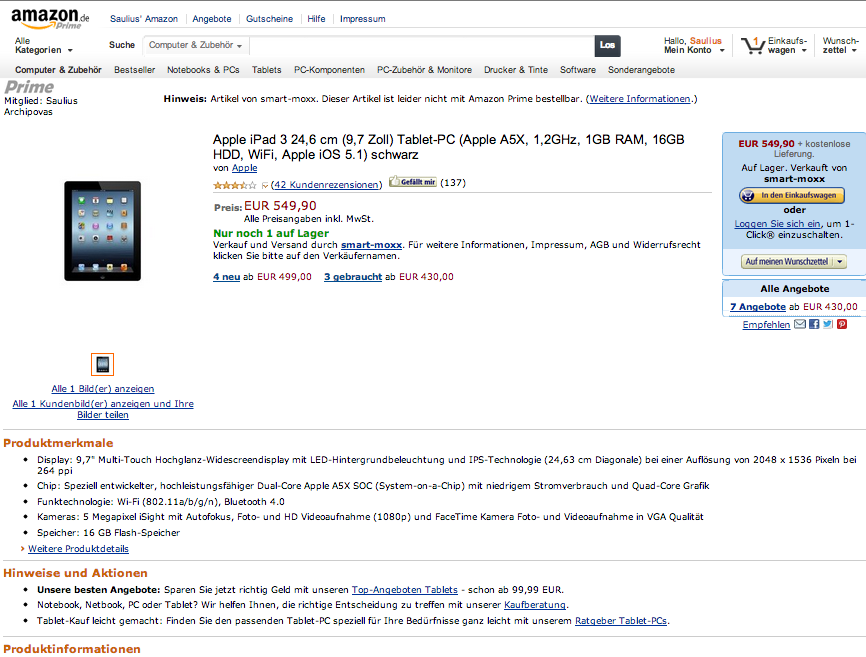
\includegraphics[width=1\textwidth]{img/amazonFull.png}
		\caption{Normale Webseite}\label{fig:amazonFull}
	\end{subfigure}
	\caption{Desktop Webseiten von Amazon}\label{fig:amazonSites}
\end{figure}

\subparagraph{Mehr Inhalt, weniger Navigation} 
\label{subp:entferne_das_fett} 

Auch die Konzentration auf den Inhalt und nicht die Navigation selbst sollte im mobilen Kontext beachtet werden\cite[Seite 52]{mobileFirst}. So hat der Besucher der Kategorie "Suche" oder "Erforschen/Spielen"  wenig Zeit um den Inhalt zu konsumieren, daher sollte er nicht mit einer Sitemap überfordert werden um zu überlegen wo er jetzt hin soll. Als gutes Beispiel dient hier die Youtube App, die einen bequemen direkten Einstieg für den Medienkonsum aufweist. Es werden Videos für den Benutzer vorgeschlagen (siehe Abbildung~\ref{fig:youtube}), was einen schnellen Inhaltskonsum verbessert. Die Seitennavigation ist unter nur einem Bedienknopf unterlegt. Somit spart dies auch Platz auf der Benutzeroberfläche.

\begin{figure}[!htb]
\minipage{0.49\textwidth}
  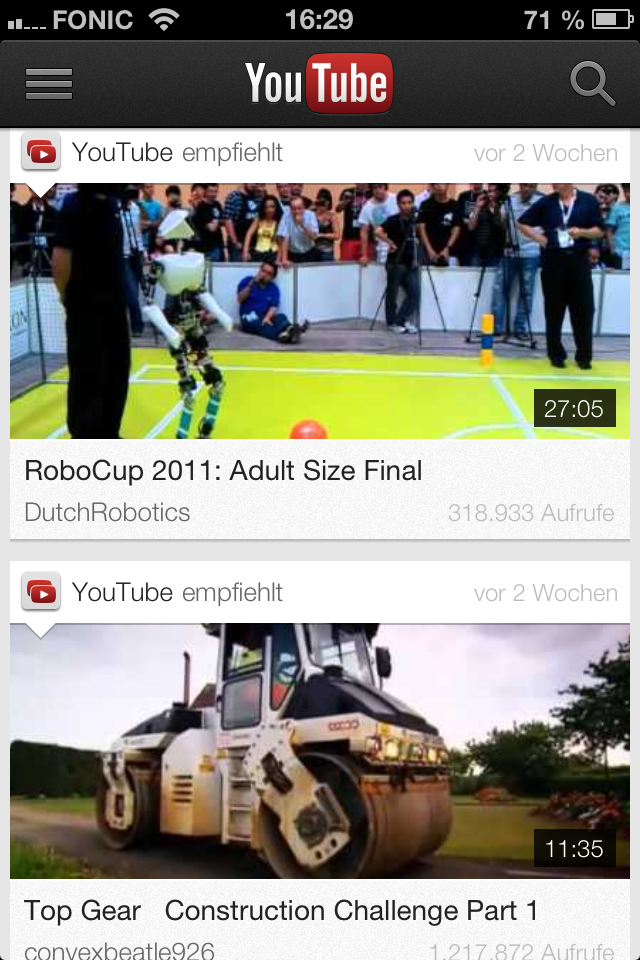
\includegraphics[width=1\textwidth]{img/youtube.png}
  \caption{Youtube App}\label{fig:youtube}
\endminipage\hfill
\minipage{0.49\textwidth}
  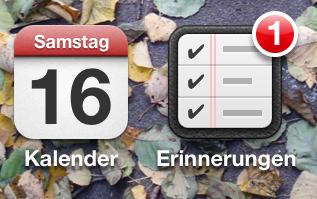
\includegraphics[width=1\textwidth]{img/iconIos.png}
	\caption{Schneller Zugriff auf Informationen}\label{fig:iconIos}
\endminipage
\end{figure}
\subparagraph{Schneller Zugriff auf wichtige Informationen} 
\label{subp:subparagraph_name}

Wie im Szenario "Suche", will der Benutzer nicht immer in das Innenleben von Programmen eintauchen, nur um einen kleinen wichtigen Bruchteil der Information zu gewinnen. Deshalb sollten wesentliche Informationen schon beim Überblick erkennbar sein(vgl. \cite[Seite 54]{mobileFrontier} und \cite{Neil:2012uf}). Als Beispiel dient z. B. die iPhone Startansicht. Hier wurden die Piktogramme so gestaltet, dass sie wichtige Information selbst beinhalten. So beinhaltet etwa die Piktogramm von iOS Kalender den heutigen Tag, oder die Erinnerungs App Hinweise auf die Anzahl der Erinnerungen (siehe Beispiel in Abbildung~\ref{fig:iconIos}).


\subparagraph{Reduziere kognitive Aufgaben} 
\label{subp:reduziere_kognitive_aufgaben_}

Im mobilen Kontext ist der Benutzer meistens mit verschiedenen Aufgaben beschäftigt. So ist auch die Verfügbarkeit der Aufmerksamkeit viel weniger, als etwa im Büro. Bei Gestaltung von Applikationen, mit denen in mobilen Kontexten gearbeitet werden soll, sollte dieser Umstand immer berücksichtigt werden. Es sollten daher Anwendungen entstehen, die unnötige Denkarbeit und damit Konzentrationsbedarf abnehmen. Zum Beispiel können die typischen "Wo bin ich gerade" Hinweise angezeigt werden, oder eine klare Strukturierung der Navigation sowie des Layouts viel in reizüberfluteten Umgebungen helfen. 

Auch die Elemente der Benutzeroberfläche dürfen den Benutzer nicht überfordern. So sollten unnötige Animationen in einer Applikation vermieden werden, da sie den Anwender unnötig ablenken oder seine Aufmerksamkeit für längere Zeit in Anspruch nehmen als nötig. Solche Ablenkungen können den Nutzer sogar gefährden, da er von seiner Tätigkeiten in der realen Welt abgelenkt ist. Ein typisches Beispiel hierfür sind Unfälle, die z.B. bei Spaziergängen auftreten können (vgl. \cite{Nasar:2008cc}).

\subparagraph{Reduzierung der Navigationstiefe} 
\label{subp:reduziere_das_w_hlen}

Eine hierarchisch aufgebaute Navigation ist ein viel benutztes Navigationsmuster in Webseiten sowie Desktop Applikationen. Dieses Muster sollte auch für Applikationen im mobilen Kontexten benutzt werden. Dabei muss beachtet werden dass die Tiefe der Navigation nichts zu groß ist. Denn mit jeder weiteren Tiefe muss der Benutzer sich an mehr erinnern und mehr abrufen. Dies ist im mobilen Kontext schwierig, weil er oft abgelenkt wird und so meistens nur 4 Sekunden Aufmerksamkeitsspanne auf die Applikation hat\cite{Oulasvirta:2005vn}. In nicht mobilen Kontexten wurde beobachtet, dass bei hierarchisch aufgebauten Navigationen die Fehleranfälligkeit beim Navigieren von 4\% bei einer Stufe auf 34.0\% bei 6 Stufen steigt, (Snowberry at al. Zitiert von \cite{Chae:2004gp}). Diese Beobachtung sollte in Betracht gezogen werden, und so auch in mobilen Kontexten die Tiefe der Hierarchie nicht höher als 3 Stufen angelegt werden.

\subparagraph{Nutzung alternativer Ein- und Ausgabequellen}
\label{subp:nutze_alternative_eingabenger_ten}

Die Interaktion mit mobilen Gerät kann in einem mobilen Kontext durch vieles beeinflusst werden. So darf der Benutzer etwa beim Fahren einen Autos das Smartphone nicht mit der Hand bedienen und der Blick kann nicht immer auf den Bildschirm gerichtet werden. So sollten auch andere Ein- oder Ausgabequellen benutzt werden. Im Auto kann dies z.B. die Sprache sein.

Auch die Geolokalisierung kann sehr behilflich sein. Etwa um dem Benutzer Informationen anzubieten, wenn er einen bestimmten Ort erreicht ohne diesen vorher in seine Applikation eingegeben zu haben. Eine Geolokalisierung kann dem Benutzer auch helfen, bei einer Suche nur die Informationen zu erhalten, die relevant für den Ort sind, an dem er sich gerade befindet. Ein Beispiel wäre hier die Suche nach einem Kaffee. Mit Hilfe der Geolokalisierung können nur die Kaffees angezeigt werden, die sich in unmittelbarer Nähe befinden und nicht alle Kaffees aus z.B. der ganzen Welt. 

Die Benutzung von Status-Led oder Vibration kann den Benutzer auf Ereignisse Hinweisen, ohne dass er immer auf den Bildschirm schauen muss. So kann man in Android Notifications API benutzen, um etwa die Status-LED in bestimmten Farbe und Intervallen blinken zu lassen (vgl. \cite{androidNotApi}). Benachrichtigungen bergen aber auch viele Gefahren, wenn sie nicht durchdacht benutzt werden. So kann es leicht passieren, dass der Benutzer mit Benachrichtigungen regelrecht überflutet wird und sich nicht mehr auf die Erfüllung seiner gewünschten Aufgaben konzentrieren kann, da er permanent von Benachrichtigungen abgelenkt wird.

\subparagraph{Gestaltung für Unterbrechungen}
\label{subp:erm_gliche_eine_fortsetzung}

In mobilen Kontexten wird der Benutzer oft in der Interaktion mit einem mobilen Gerät unterbrochen oder er hat nicht genügend Zeit seine Aufgaben zu beenden. Es sollten daher Möglichkeiten angeboten werden, die Aufgaben später zu erledigen. So sollten etwa Benutzereingaben oder Anwendungszustand nach einer bestimmten Zeit der Nichtnutzung nicht zurückgesetzt werden um dem Benutzer eine Fortsetzung seiner Aufgabe zu ermöglichen.

Die Hersteller von mobilen Betriebssystemen bieten hierfür spezielle APIs, um dies zu ermöglichen. So können Daten beim Schließen der Applikation zwischengespeichert werden, um nach dem nächsten Aufruf  weiter ausgeführt werden zu können. Wenn der Benutzer dies nicht wünscht, sollte es aber eine Möglichkeit geben, die Applikation mittels weniger Interaktionen in den Startzustand zurückzusetzen.

Außerdem solle man dem Benutzer die Möglichkeit geben, bei bestimmten Kontexten Teilaufgaben zu markieren, um sie später bearbeiten zu können. Als gutes Beispiel dient hier der Dienst "Pocket" \footnote{Vorher als "Read it later" bekannt, http://getpocket.com }. Hier kann der Benutzer in einer ersten Durchsicht interessante Artikeln, oder Webseiten markieren, um sie später in aller Ruhe durchlesen zu können. Ein anderes Beispiel sind Dienste, mit denen man gerade besuchte Orte markieren kann, um danach mehr Information über diese zu erfahren.

\subparagraph{Fokussierung auf Erfahrungen, die nur mobil auftreten können} % (fold)
\label{subp:fokussiere_auf_erfahrungen_die_nur_mobil_auftreten_k_nnen}

In diesem Kapitel wurden vier Kategorien eingeführt, die die Art der Interaktion mit dem mobilen Endgerät beschreiben. Die Anwendungen für den mobilen Kontext sollten diese daher auch bedienen, und nicht versuchen einen stationären Arbeitsplatz zu imitieren. Auch die Erfahrungen, die nur mobil auftreten können, sollten berücksichtigt werden. 

Zum Beispiel sollte eine Notiz Applikationen dem Benutzer ermöglichen, Lokalisierungsinformationen oder Schnelle Schnappschüsse zu speichern. Oder eine Applikation, die Preisvergleiche macht, sollte eine Barcode-Lesefunktion haben, um dem Benutzer beim Besuch eines Ladens zu ermögliche, die Preise zu scannen.  Auch eine Rabattcoupon-Erinnerung bei Besuchen eines bestimmten Laden könnte dem Benutzer Freude an der Applikation bereiten (vgl. \cite{smartOnline})
\newline

In diesem Teilkapitel wurden die vier Arten der Interaktion, sowie wichtige Hinweise für die Erstellung von Applikationen hinsichtlich ihre Informationsarchitektur gegeben. So wurde empfohlen die Applikationen nicht mit zu viel Text, Funktionalitäten und Navigationstiefe zu überfrachten um den Benutzer nicht zu überfordern. Stattdessen sollte sich mehr auf den knappen und schnell für den Benutzer aufrufbaren wichtigen Inhalt konzentrieren werden. 
In nächsten Teilkapitel werden Hinweise zur Gestaltung von Diensten gegeben.

\subsection{Gestaltung von Diensten}
\label{sub:gestaltung_von_diensten}

Nicht nur das visuelle Design der Applikation muss für den mobilen Einsatz angepasst werden, sondern auch die Dienste, die die Applikation anbietet, sollten den mobilen Einsatz unterstützen. 

Bis jetzt wurden die Kernaufgaben, die mit einem Rechner erledigt werden konnten, mit dem stationären Rechner erledigt. Mit der immer mehr verbreiteten Benutzung von mobilen Geräten, sollten die Barrieren des Informationsaustauschs zwischen den beiden Gerätearten abgebaut werden. Als Benutzer will man eine Möglichkeit, Arbeiten die an einem Gerät angefangen wurden, auf dem anderen Gerät weiterzuführen. Diese Bedürfnisse wurden teils von Mitarbeitern aus dem precious design studio analysiert und es wurden sechs Beziehungsmuster von Anzeigen identifiziert, die auch für Gestaltung von Diensten benutzt werden könnten\cite{slideEcosystems}. Im Folgenden werden die Beziehungsmuster Kohärenz, Synchronisation und Gerätemobilität näher betrachtet.

\subparagraph{Kohärenz}

Dienste, die auf einem stationären Rechner laufen, sollten auch die Möglichkeit bieten die Hauptfunktionalität des Dienstes auf einem mobilen Gerät zu benutzen. So soll auch eine sofortige Synchronisation zwischen Geräten existieren, die  Bearbeitung von Aufgaben auf einem beliebigen Gerät zu ermöglichen. Dabei soll Applikation die Vorteile des jeweiligen Geräts Nutzen.

Als gutes Beispiel dient hier die Anwendung Evernote, die für Notizen benutzt werden kann. So kann man mit dem mobilen Gerät Notizen oder Photos hochladen und sie nachher weiter an jedem beliebigen Rechner bearbeiten oder vice versa. Um die Vorteile von mobilen Gerät auszunutzen, werden etwa Daten vom Aufnahmeort zu jeder Notiz abgespeichert. Außerdem ist die mobile Applikation für Foto-, Audio- und Videonotizen optimiert. So wird durch abfotografieren von Textpassagen der Text erkannt und ins Maschinelle übersetzt. Damit wird die unproduktive Eingabe eines Textes auf einem mobilen Gerät umgangen.

\subparagraph{Synchronisation}

Benutzer erwarten zunehmend, dass die digitalen Informationen und Daten von überall aufrufbar sind. Dies kann gelöst werden, indem man die Daten zwischen den Geräten synchronisiert, ohne dass dies explizit vom Anwender initiiert wird. So kann der Benutzer bei einem Wechsel des Gerätes auf identische Daten zugreifen. 

Als Beispiel dient hier die iCloud von Apple. Hier werden Termine, Musik, Fotos oder Bücher zwischen den Geräten synchronisiert und auf dem neusten Stand gehalten. Beim Amazon Kindle Dienst ist es möglich nicht nur gleiche Bücher auf verschieden Geräten zu haben, sondern das Lesen auch auf der gleichen Seite des Buchs fortzuführen, bei der auf dem anderen Gerät das Lesen beendet wurde.

\subparagraph{Gerätemobilität}

Bei der Interaktion mit den Gerät kann es passieren, dass sich die Intention des Anwenders oder die Umgebung in der Weise ändert, dass das gerade benutzte Gerät nicht mehr dessen Bedürfnisse erfüllen kann und die Nutzung der Informationen auf einen anderes Gerät ausgelagert wird. Dabei soll dem Benutzer dabei geholfen werden, Informationen auf ein Gerät ohne großen Aufwand zu übertragen, zu verschieben, umzuschalten, zu verlagern oder zu hinterlegen.

\begin{figure}[h]
\centering
  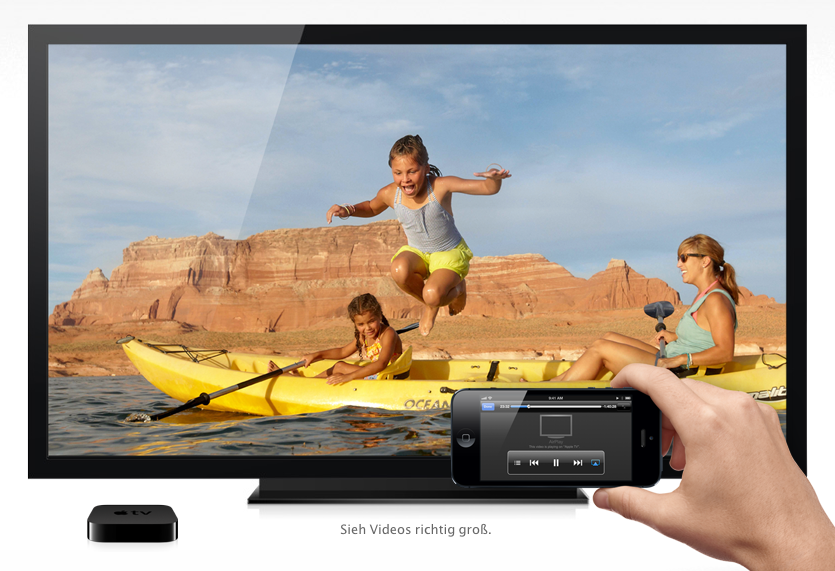
\includegraphics[width=1\textwidth]{img/airplay.png}
  \caption{Airplay, Bild aus \cite{airplaySite}}\label{fig:airplay}
	
\end{figure}
Als gutes Beispiel dient hier Apple AirPlay. Damit kann der Benutzer auf dem iPhone oder iPad angefangene Filme oder Musik, auf ein anderes Gerät, das AirPlay unterstützt, verlagern. So kann z.B. der  Film sofort auf dem verlagerten Gerät weitergespielt werden, siehe Abbildung~\ref{fig:airplay}
\newline

In diesem Kapitel wurden drei Muster für die Gestaltung von Diensten für den mobilen Kontext vorgestellt, die den Benutzer den Wechsel zwischen verschiedenen  Endgeräten erleichtern sollen. Im nächsten Kapitel werden spezielle Anforderungen bei Wearable Computing aufgezeigt, um einen breiteren Überblick über Design im mobilen Kontext zu geben.

\subsection{Spezielle Anforderungen bei Wearable Computing} 
\label{sub:wearable_computers}


Wearable Computing, oder tragbare Datenverarbeitung, ist das Forschungsgebiet, das sich mit der Entwicklung von tragbaren Computersystemen (Wearable Computers) beschäftigt\cite{wikiWearable}. So wird versucht, alltägliche Aktivitäten oder Bedürfnisse des Benutzers  mit Hilfe von Computersystemen zu erleichtern oder auch erst zu ermöglichen. Dabei tritt aber das Computersystem in den Hintergrund. Die Geräte können von beliebiger Form sein und jede beliebige Funktion erfüllen: Die Möglichkeiten reichen hier z.B. von einer Armbanduhr, die ähnlich den Smartphone funktioniert (vgl. \cite{zeitPc}) bis hin zu  einem  Ring, der den Puls sowie den Sauerstoffgehalt im Blut misst (vlg. \cite{urhWearable}).  Um die Einführung in die Gestaltungsprinzipien des Wearable Computing kurz zu halten, konzentriert sich dieses Kapitel auf die Benutzung von Wearable Computing im Arbeitsumfeld, auf die Forschung in TZI Wearable Labs sowie auf Head-Up-Display (HUD) Ausgabegeräte.

Wearable Computing kann unter auch das Arbeiten in der Industrie (Wartungs-, Lagerarbeit), in der Gesundheitspflege und in anderen Bereichen erleichtern \cite{Witt:2006hi},\cite{Lawo:2008gg}. So besteht eine typische Arbeitskleidung aus einem HUD, einer tragbaren Tastatur sowie einem Handschuh mit Steuerungskomponenten. Die Ausgabe von den Computern kann mittels eines Displays in einem HUD benutzt werden, und die Eingabe mittels einer Tastatur sowie einem Steuerungshandschuh erfüllt werden. 

Anders als in stationären Arbeitsumfeldern, wo meistens nur eine Hauptaufgabe an einem Rechner bearbeitet wird, wird in Wearable Computing erwartet, dass der Benutzer zwei Aufgaben erfüllt \cite{Witt:2006hi}. Diese Aufgaben können in primäre und sekundäre Aufgaben eingeteilt werden. Die primäre Aufgabe besteht meistens aus einer Interaktion mit der Umwelt, etwa dem Drehen einer Schraube oder dem Scannen eines Paketes. Primäre Aufgaben können durch die Benutzung von tragbaren Computersystemen erleichtert werden, indem sie diese als sekundären Aufgaben einteilen. Sekundäre Aufgaben wären etwa die Bestätigung nach dem Einschrauben einer Schraube oder eine visuelle Information über ein gerade eingescanntes Paket. Falls eine sekundäre Aufgaben existiert und erledigt werden muss, soll dabei der Benutzer nicht zu sehr von der primären Aufgabe ablenkt werden. Daher muss er auf adäquate Weise auf die sekundäre Aufgabe aufmerksam gemacht werden. Um die Aufmerksamkeit des Benutzers auf die sekundäre Aufgabe zu lenken, können 4 Benachrichtigungssysteme benutzt werden: "sofortige", "verhandelbare", "vermittelte" und "geplante" Benachrichtungungen (vlg. \cite{McFarlane:1999um},\cite{Nilsson:cq}). Bei der sofortigen Benachrichtigung, wird der Benutzer sofort über neue Informationen informiert. Solche Benachrichtigungen sind etwa nützlich bei der Betreuung von Auszubildenden in Autowerkstätten die durch einen Computer koordiniert wird. So können anhand eines Arbeitsschritts, die benötigten Werkzeuge auf den HUD angezeigt werden. Falls eine Schraube am falschen Ort befestigt wurde, wird  der Benutzer so sofort informiert. Bei verhandelbare Benachrichtigungssysteme wird der Anwender über ein Ereignis auf seinem HUD und kann dann selber entscheiden, ob er auf dieses regieren will. So kann etwa der Lagerarbeiter beim Eintreffen neuer Pakete im Lager informiert werden, und somit entscheiden ob er die dafür anfallenden Tätigkeit sofort erledigen möchte. Bei einer "vermittelten" Benachrichtigung, können andere Arten der Ausgabe für Benachrichtigungen verwendet werden, die nicht so aufdringlich sind wie die Anzeige auf einem HUD. Ein Beispiel hierfür wäre eine Audiodatei, die abgespielt wird um den Benutzer über ein Ereignis zu informieren. Falls der Benutzer darauf Reagieren möchte, kann er  dies mittels eines Eingabegerätes tun. Bei "geplanten" Benachrichtigungen werden die Aufgaben  akkumuliert und in festgelegten Intervallen angezeigt. In der Studie \cite{Nilsson:cq}  haben "geplante" Benachrichtigungssysteme sowohl bei der Effizienz als auch bei der subjektiven Meinung der Probanden,  am besten abgeschnitten. Dies sollte bei der Entwicklung von Anwendungen in Betracht gezogen werden.


In diesem Kapitel wurde mehrere Hinweise, die für die Gestaltung von Diensten, Benutzeroberflächen sowie Funktionalitäten für Anwendungen im mobilen Kontext benutzt werden sollten erläutert. Im nächsten Kapitel wird eine Beispielanwendung vorgestellt und analysiert.

